\label{extractevents}
\section{Introduction}
To isolate individual events such as EPSCs or EPSPs from recorded data, Stimfit uses a\keyindex{templatematching}{event detection!template matching}{template matching}\index{template matching|see{event detection}} template matching algorithm as decribed by \citetext{Jonas93}, with some implementation details adopted from \citetext{Clements97}. The template consists of a waveform $p(t)$ with a length of $n$ sampling points that represents the time course of a typical event. The template is slid over the trace of recorded values $r(t)$, and at each sampling point with index $s$, it is multiplied by a scaling factor $m$ and an offset $c$ is added or subtracted so that the sum of squared errors $\chi^2(t_s)$ between the trace and the template is minimised:
\begin{equation*}
  \chi^2(t_s)=\sum_{k=0}^{n-1}\left[r(t_{s+k})-\left(m{\cdot}p(t_k)+c\right)\right]^2
\end{equation*}
As can be seen from this equation, this amounts to the fairly simple operation of fitting a straight line that relates $p(t)$ and $r(t)$ at every sampling point.

Finally, some \keyindex{detectioncriterion}{event detection!detection criterion}{detection criterion}\index{detection criterion|see{event detection}}detection criterion has to be applied to decide whether an event has occurred at a sampling point. Two options are available in Stimfit: \citetext{Jonas93} suggest to use the linear correlation coefficient between the optimally scaled template and the data, whereas \citetext{Clements97} compare the scaling factor with the noise standard deviation.

\section{A practical guide to event detection}
In practice, the following steps need to be performed to extract events with Stimfit:
\begin{enumerate}
 \item Create a preliminary template by fitting a function to a single, large and isolated event.
 \item Use this preliminary template to extract some more examplary large and isolated events using a high detection criterion threshold.
 \item Create the final template by fitting a function to the average of the exemplary events.
 \item Extract all events with the final template using a low detection criterion threshold.
 \item Eliminate false-positive, add false-negative events.
\end{enumerate}
This procedure will be explained in some more detail in the following sections.

\subsection{Create a preliminary template}
In general, the template waveform $p(t)$ can be of arbitrary shape. A typical way of creating such a template is to fit a function with a time course matching the event kinetics to some exemplary events. For example, EPSCs can typically be modelled with the sum or the product of two exponential functions \footnote{Note that the product of two exponentials $f(t)=a\left(1-e^{-\frac{t}{\tau_1}}\right)e^{-\frac{t}{\tau_2}}$ can equivalently be expressed as the sum of two exponentials: $f(t)=a\left(e^{-\frac{t}{\tau_2}}-e^{-\frac{t}{\tau_3}}\right)$, with $\tau_3=\frac{\tau_1\tau_2}{\tau_2-\tau_1}$.}. In practice, a robust estimate for a template can be obtained using an iterative approach, which will be illustrated here using a recording of miniature EPSCs that you can download \href{http://stimfit.org/tutorial/minis.dat}{here}\footnote{\url{http://stimfit.org/tutorial/minis.dat}}.

\label{bait}First, we fit a function to a single large and isolated event to create a preliminary ``bait'' template.
  \begin{myfigure}[htb]
    \begin{center}
      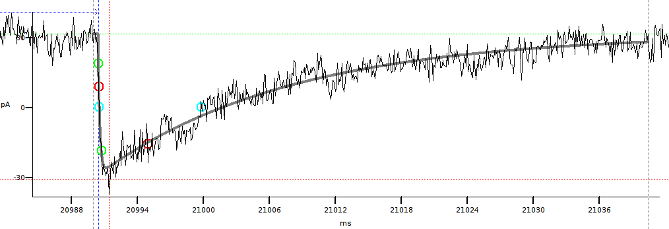
\includegraphics[scale=0.41]{./img/bait_template.eps}
    \end{center}
    \caption{Creation of a ``bait'' template.}
    \label{baittemplate}
  \end{myfigure}
In this case, we will use the EPSC that can be found roughly between \textit{t}~=~20990~ms and \textit{t}~=~21050~ms. Then, we fit the sum of two exponential functions with a delay to this EPSC. To obtain the same template as in the example, you can call the function \pycommand{preliminary} from the \pycommand{minidemo} module that comes bundled with stimfit:
\begin{lstlisting}
>>> import minidemo
>>> minidemo.preliminary()
\end{lstlisting}
This will take care of the appropriate cursor positions and the biexponential fit (see p. \pageref{setpeakstart} for setting the cursors from Python, and p. \pageref{leastsq} for the \pycommand{leastsq} function). If you prefer, you can use the fit settings dialog as described in chapter \ref{gettingstarted} (Fig. \ref{fitselection}, p. \pageref{fitselection}).

\subsection{Extract exemplary events}
We now use the bait template to fish some more large and isolated events. Choose ``Analysis''$\rightarrow$``Event detection'' $\rightarrow$``Template matching...'' from the menu.
  \begin{myfigure}[htb]
    \begin{center}
      \includegraphics[scale=0.5]{./img/event_dialog.eps}
    \end{center}
    \caption{Event detection settings.}
    \label{eventdialog}
  \end{myfigure}
In the dialog that will pop up (Fig. \ref{eventdialog}), you can set the threshold for the detection criterion. Since we want to extract some large and isolated events during this first pass, we set this to a high number, say 10, using the template scaling factor \cite{Clements97}. Click ``OK'' to start the event detection. When finished, press \keybox{F} to fit the whole trace to the window. The detected events will be marked by blue arrows in the upper part of the window, and blue circles will indicate the peak values of the detected events (Fig. \ref{events}).
  \begin{myfigure}[htb]
    \begin{center}
      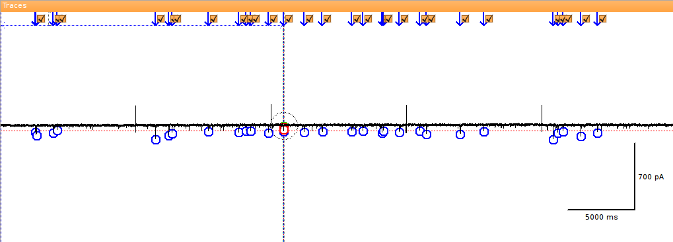
\includegraphics[scale=0.4]{./img/events.eps}
    \end{center}
    \caption{Detected events.}
    \label{events}
  \end{myfigure}
To view the isolated events in a new window, you have to switch to the event editing mode, either by pressing \keybox{E} or by activating the corresponding button in the toolbar (Fig. \ref{eventbutton}).
  \begin{myfigure}[htb]
    \begin{center}
      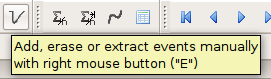
\includegraphics[scale=0.5]{./img/eventbutton.eps}
    \end{center}
    \caption{Switching to event editing mode.}
    \label{eventbutton}
  \end{myfigure}
When you now click on the trace with the right mouse button, a menu will show up. Select ``Extract selected events'' from this menu. This will put the exemplary EPSCs into a new window.

\subsection{Create the final template}
We now create the average of all extracted events, as explained in chapter \ref{gettingstarted} (p. \pageref{averagecalculation}). Then, we fit a biexponential function to the average, as explained above for the single EPSC (see p. \pageref{bait}). Remember to set the baseline, peak and fit window cursors appropriately before performing the fit, and to update all calculations. Again, you can make use of a function from the \pycommand{minidemo} module to set the cursors and perform the fit:
\begin{lstlisting}
>>> import minidemo # if you haven't imported it already
>>> minidemo.final()
\end{lstlisting}
The final template should look similar as shown in Fig. \ref{finaltemplate}.
  \begin{myfigure}[htb]
    \begin{center}
      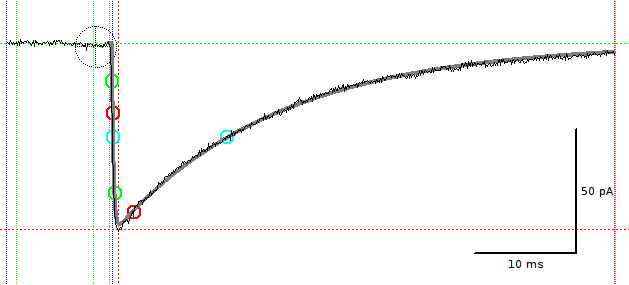
\includegraphics[scale=0.5]{./img/finaltemplate.eps}
    \end{center}
    \caption{Creating a final template.}
    \label{finaltemplate}
  \end{myfigure}

\subsection{Extract all events}
Go back to the original file (minis.dat). Extracting all events with the final template is done in nearly the same way as described above for the preliminary template. However, you have to choose the correct template in the event dialog: The final template in this case is the second on the list (Fig. \ref{selectfinal}).
  \begin{myfigure}[htb]
    \begin{center}
      \includegraphics[scale=0.5]{./img/selectfinal.eps}
    \end{center}
    \caption{Selecting the final template.}
    \label{selectfinal}
  \end{myfigure}
For this final run, we will lower the detection threshold to a value of 3, as suggested by \citetext{Clements97}.

\subsection{Edit detected events}
Usually, the detected events have to be screened visually to remove false-positives and add false-negatives. Removing false positives is done by unselecting the checkbox next to the arrow indicating an event (Fig. \ref{events}). To add false-negatives, you have to switch to the event-editing mode (Fig. \ref{eventbutton}) and then right-click on the trace at the position where the event starts. From the context menu that will pop up, select ``Add an event that starts here'' (Fig. \ref{falsenegative}). To efficiently screen the whole trace, it is convenient to use \keybox{Shift} and \keybox{$\leftarrow$} at the same time. This will move the trace left by the width of one window. Once you are done with editing, choose ``Extract selected events'' from the context menu.
  \begin{myfigure}[htb]
    \begin{center}
      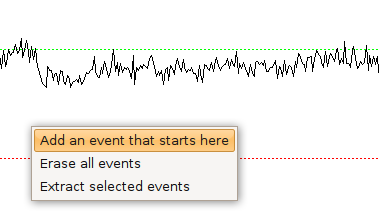
\includegraphics[scale=0.5]{./img/falsenegative.eps}
    \end{center}
    \caption{Adding a false-negative event.}
    \label{falsenegative}
  \end{myfigure}

\subsection{Analyse extracted events}
If you used the same settings as suggested above, 97 events will be extracted. You will find a table on the left of the traces: This will show you the time of onset of the events and the inter-event intervals. Usually, you will want to apply some further analysis to the extracted events. To do so, you first have to adjust the baseline, peak and fit cursors. Again, there is a function in the \pycommand{minidemo} module taking care of that:
\begin{lstlisting}
>>> minidemo.batch_cursors()
\end{lstlisting}
To analyse all traces efficiently, you can now perform a \keyindex{batchanalysis}{batch analysis}{batch analysis}``batch analysis'' on all traces at once: First, select all traces, either using \pycommand{select\_all()} from the shell (see p. \pageref{selectall}) or ``Edit''$\rightarrow$``Select all traces'' from the menu or pressing \keybox{Ctrl} and \keybox{A} at the same time. Then, choose ``Analysis''$\rightarrow$``Batch analysis'' from the menu.
  \begin{myfigure}[htb]
    \begin{center}
      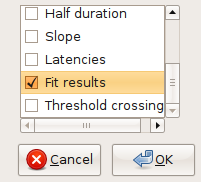
\includegraphics[scale=0.5]{./img/batchanalysis.eps}
    \end{center}
    \caption{Batch analysis settings.}
    \label{batchanalysisdlg}
  \end{myfigure}
From the dialog (Fig. \ref{batchanalysisdlg}), choose the analysis functions that you want to apply to your data. Click ``OK'' once you are done. A new table will appear to the left of the traces. You can copy and paste values from the tables to spreadsheet programs for further analysis.

\subsection{Adjusting event detection settings}
\small
\begin{tabular}{p{0.45\textwidth} p{0.45\textwidth}}
\textit{Problem} & \textit{Solution} \\ \hline 
 & \\
Too many false-positive events have been detected & Increase the detection threshold \\
 & \\
Too many events have been missed (false-negatives) & Decrease the detection threshold \\
 & \\
One and the same event is detected multiple times at short time intervals & Increase the number of sampling points between events \\
 & \\
Closely spaced events are not detected separately & Decrease the number of sampling points between events \\
\end{tabular}
